%\VignetteIndexEntry{homals} 

\documentclass[article]{jss1}
\usepackage{amsmath, amsfonts}
\usepackage{float,amssymb}
\usepackage{hyperref}


\newcommand{\defi}{\mathop{=}\limits^{\Delta}}  
%%%%%%%%%%%%%%%%%%%%%%%%%%%%%%
%% declarations for jss.cls %%%%%%%%%%%%%%%%%%%%%%%%%%%%%%%%%%%%%%%%%%
%%%%%%%%%%%%%%%%%%%%%%%%%%%%%%

%% almost as usual
\author{Jan de Leeuw\\University of California, Los Angeles \And 
        Patrick Mair \\Wirtschaftsuniversit\"at Wien}
\title{Gifi Methods for Optimal Scaling in R:\\ The Package \pkg{homals}}
%
%%% for pretty printing and a nice hypersummary also set:
\Plainauthor{Jan de Leeuw, Patrick Mair} %% comma-separated
\Plaintitle{Gifi Methods for Optimal Scaling in R: The Package homals} %% without formatting
\Shorttitle{Homals in \proglang{R}} %% a short title (if necessary)

%% an abstract and keywords
\Abstract{
Homogeneity analysis combines maximizing the correlations between variables of a multivariate data set with
that of optimal scaling. In this article we present methodological and practical issues of the \proglang{R} package \pkg{homals} which performs homogeneity analysis and various extensions. By setting rank constraints nonlinear principal component analysis can be performed. The variables can be partitioned into sets such that homogeneity analysis is extended to nonlinear canonical correlation analysis or to predictive models which emulate discriminant analysis and regression models. For each model the scale level of the variables can be taken into account by setting level constraints. All algorithms allow for missing values.
}
\Keywords{Gifi methods, optimal scaling, homogeneity analysis, correspondence analysis, nonlinear principal component analysis, nonlinear canonical correlation analysis, homals, \proglang{R}}
\Plainkeywords{Gifi methods, optimal scaling, homogeneity analysis, optimal scaling, correspondence analysis, nonlinear principal component analysis, nonlinear canonical correlation analysis, homals, R} %% without formatting
%% at least one keyword must be supplied

%% publication information
%% NOTE: This needs to filled out ONLY IF THE PAPER WAS ACCEPTED.
%% If it was not (yet) accepted, leave them commented.
%% \Volume{13}
%% \Issue{9}
%% \Month{September}
%% \Year{2004}
%% \Submitdate{2004-09-29}
%% \Acceptdate{2004-09-29}

%% The address of (at least) one author should be given
%% in the following format:
\Address{
 Jan de Leeuw\\
 Department of Statistics\\
  University of California, Los Angeles\\
  E-mail: \email{deleeuw@stat.ucla.edu}\\
  URL: \url{http://www.stat.ucla.edu/~deleeuw/}
}
%% It is also possible to add a telephone and fax number
%% before the e-mail in the following format:
%% Telephone: +43/1/31336-5053
%% Fax: +43/1/31336-734

%% for those who use Sweave please include the following line (with % symbols):
%% need no \usepackage{Sweave.sty}

%% end of declarations %%%%%%%%%%%%%%%%%%%%%%%%%%%%%%%%%%%%%%%%%%%%%%%


\begin{document}
\section{Introduction}
\label{sec:int}
During the last years correspondence analysis (CA) has become a popular descriptive statistical method to analyze categorical data \citep{Benzecri:73, Greenacre:84, Gifi:90, Greenacre+Blasius:06}. Due to the fact that the visualization capabilities of statistical software have increased during this time, researchers of many areas apply CA and map objects and variables (and their respective categories) onto a common metric plane. 

Currently, \proglang{R} \citep{R:07} offers a variety of routines to compute CA and related models. An overview of corresponding functions and packages is given in \citet{Mair+Hatzinger:07}. The package \pkg{ca} \citep{Nenadic+Greenacre:06} is a comprehensive tool to perform simple and multiple CA. Various two- and three-dimensional plot options are provided.  

In this paper we present the \proglang{R} package \pkg{homals}, starting from the simple homogeneity analysis, which corresponds to a multiple CA, and providing several extensions. \citet{Gifi:90} points out that homogeneity analysis can be used in a \emph{strict} and a \emph{broad} sense. In a strict sense homogeneity analysis is used for the analysis of strictly categorical data, with a particular loss function and a particular algorithm for finding the optimal solution. In a broad sense homogeneity analysis refers to a class of criteria for analyzing multivariate data in general, sharing the characteristic aim of optimizing the homogeneity of variables under various forms of manipulation and simplification \citep[p. 81]{Gifi:90}. This view of homogeneity analysis will be used in this article since \pkg{homals} allows for such general computations. Furthermore, the two-dimensional as well as three-dimensional plotting devices offered by \proglang{R} are used to develop a variety of customizable visualization techniques.    
More detailed methodological descriptions can be found in \citet{Gifi:90} and some of them are revisited in \citet{Michailidis+deLeeuw:98}. 


\section{Homogeneity Analysis}
In this section we will focus on the underlying methodological aspects of \pkg{homals}. Starting with the formulation of the loss function, the classical alternating least squares algorithm is presented in brief and the relation to CA is shown. Starting from basic homogeneity analysis we elaborate various extensions such as nonlinear canonical analysis and nonlinear principal component analysis. A less formal introduction to Gifi methods can be found in \citet{Mair+deLeeuw:2008}. 

\subsection{Establishing the loss function}
Homogeneity analysis is based on the criterion of minimizing the departure from homogeneity. Homogeneity is measured by a loss function. To write the corresponding basic equations the following definitions are needed. For $i=1,\ldots,n$ objects, data on $m$ (categorical) variables are collected where each of the $j=1,\ldots,m$ variable takes on $k_j$ different values (their \emph{levels} or \emph{categories}). We code them using $n\times k_j$ binary \emph{indicator matrices} $G_j$, i.e., a dummy matrix for each variable. The whole set of indicator matrices can be collected in a block matrix
\begin{equation}
G\defi\begin{bmatrix}G_1&\vdots&G_2&\vdots&\cdots&\vdots&G_m\end{bmatrix}.
\end{equation}
In this paper we derive the loss function including the option for missing values. For a simpler (i.e. no missings) introduction the reader is referred to \citet[][p. 307--314]{Michailidis+deLeeuw:98}. In the indicator matrix missing observations are coded as complete zero rows; if object $i$ is missing on variable $j$, then row $i$ of $G_j$ is 0, otherwise row sum becomes 1 since the category entries are disjoint. This corresponds to the first missing option presented in \citet[p. 74]{Gifi:90}. Other possibilities would be to add an additional column to the indicator matrix for each variable with missing data or to add as many additional columns as there are missing data for the $j$-th variable. However, our approach is to define the binary diagonal matrix $M_j$ if dimension $n \times n$ for each variable $j$. The diagonal element $(i,i)$ is equal to 0 if object $i$ has a missing value on variable $j$ and equal to 1 otherwise. Based on $M_j$ we can define $M_\star$ as the sum of the $M_j$'s and $M_\bullet$ as their average.  

For convenience we introduce
\begin{equation}
D_j^{}\defi G_j'M_j^{}G_j^{}=G_j'G_j^{},
\end{equation}
as the $k_j\times k_j$ diagonal matrix with the (marginal) frequencies of variable $j$ in its main diagonal. 

Now let $X$ be the unknown $n\times p$ matrix containing the coordinates (\emph{object scores}) of the object projections into $\mathbb{R}^p$. Furthermore, let $Y_j$ be the unknown $k_j \times p$ matrix containing the coordinates of the category projections into the same $p$-dimensional space (\emph{category quantifications}). 
The problem of finding these solutions can be formulated by means of the following loss function to be minimized:
\begin{equation}
\label{eq:loss}
\sigma(X;Y_1,\ldots,Y_m)\defi \sum_{j=1}^m\mathbf{tr}(X-G_jY_j)'M_j(X-G_jY_j)
\end{equation}
We use the normalization $\mathbf{u}'M_\bullet X=0$ and $X'M_\bullet X=I$ in order to avoid the trivial solution $X=0$ and $Y_j=0$. The first restriction centers the graph plot (see Section \ref{sec:R}) around the origin whereas the second restriction makes the columns of the object score matrix orthogonal. Multiplying the scores by $\sqrt{n/m}$ gives a mean of 0 and a variance of 1 (i.e., they are $z$-scores). Note that from an analytical point of view the loss function represents the sum-of-squares of $(X-G_jY_j)$ which obviously involves the object scores and the category quantifications. Thus, the aim is to minimize simultaneously over $X$ and $Y_j$. We give a graphical interpretation of the loss function in the following section. 

\subsection{Geometry of the loss function}
In the \pkg{homals} package we use homogeneity analysis as a graphical method to explore multivariate data sets. The \emph{joint plot} where the object scores and the category quantifications are mapped in a joint space, can be considered as the classical or standard homals plot. The category points are the centers of gravity of the object points that share the same category. The larger the spread between category points the better a variable discriminates and thus the smaller the contribution to the loss. The closeness of two objects in the plot is related to the similarity of their response patterns. A ``perfect'' solution, i.e., without any loss at all, would imply that all object points coincide with their category points. 

Moreover, we can think of $G$ as the adjacency matrix of a bipartite graph in which the $n$ objects and the $k_j$ categories ($j=1,\ldots,m$) are the vertices. In the corresponding \emph{graph plot} an object and a category are connected by an edge if the object is in the corresponding category. The loss in (\ref{eq:loss}) pertains to the sum of squares of the line lengths in the graph plot. Producing a \emph{star plot}, i.e., connecting the object scores with their category centroid, the loss corresponds to the sum over variables of the sum of squared line lengths. More detailed plot descriptions are given in Section \ref{sec:R}.


\subsection{Minimizing the loss function}
Typically, the minimization problem is solved by the iterative \emph{alternating least squares algorithm} (ALS; sometimes quoted as \emph{reciprocal averaging algorithm}). At iteration $t=0$ we start with arbitrary object scores $X^{(0)}$. Each iteration $t$ consists of three steps:
\begin{enumerate}
\item Update category quantifications: $Y_j^{(t)}=D_j^{-1}G_j'X^{(t)}$ for $j=1,\ldots,m$
\item Update object scores: $\tilde X^{(t)}=M_\star^{-1}\sum_{j=1}^m G_j^{}Y_j^{(t)}$
\item Normalization: $X^{(t+1)}=M_\star^{-\frac12}{\bf orth}(M_\star^{-\frac12}\tilde X^{(t)})$
\end{enumerate}
Note that matrix multiplications using indicator matrices can be implemented efficiently as cumulating the sums of rows over $X$ and $Y$. 

Here $\mathbf{orth}$ is some technique which computes an orthonormal basis for the column space of a matrix. We can use QR decomposition, modified Gram-Schmidt, or the singular value decomposition (SVD). In \pkg{homals} the left singular vectors of $\tilde X^{(t)}$, here denoted as $\mathbf{lsvec}$, are used. 

To simplify, let $P_j$ denote the orthogonal projector on the subspace spanned by the columns of $G_j$, i.e.,
$P_j^{}=G_j^{}D_j^{-1}G_j'$. Correspondingly, the sum over the $m$ projectors is 
\begin{equation}
P_\star=\sum_{j=1}^m P_j = \sum_{j=1}^m G_j^{}D_j^{-1}G_j'.
\end{equation}
Again, $P_\bullet$ denotes the average. By means of the $\mathbf{lsvec}$ notation and including $P_\bullet$ we can describe a complete iteration step as 
\begin{equation}
\label{eq:Xlsv}
X^{(t+1)}=\mathbf{lsvec}(\tilde X^{(t)})=\mathbf{lsvec}(M_\bullet^{-1}P_\bullet^{} X^{(t)}).
\end{equation}
In each iteration $t$ we compute the value of the loss function to monitor convergence. Note that Formula (\ref{eq:Xlsv}) is not suitable for computation, because it replaces computation with sparse indicator matrices by computations with a dense average projector. 

Computing the \pkg{homals} solution in this way is the same as performing a CA on $G$. Usually, multiple CA solves the generalized eigenproblem for the Burt matrix $C=G'G$ and its diagonal \(D\) \citep{Greenacre:84,Greenacre+Blasius:06}.
Thus, we can put the problem in Equation \ref{eq:loss} into a SVD context \citep{deLeeuw+Michailides+Wang:99}. Using the block matrix notation, we have to solve the generalized singular value problem of the form
\begin{eqnarray}
GY=M_\star X\Lambda, \\
G'X=DY\Lambda,
\end{eqnarray}
or equivalently one of the two generalized eigenvalue problems
\begin{eqnarray}
GD^{-1}G'X=M_\star X\Lambda^2, \\
G'M_\star^{-1}GY=DY\Lambda^2.
\end{eqnarray}
Here the eigenvalues $\Lambda^2$ are the ratios along each dimension of the average between-category variance and the average total variance.
Also $X'P_jX$ is the between-category dispersion for variable $j$. Further elaborations can be found in \citet{Michailidis+deLeeuw:98}. 

Compared to the classical SVD approach, the ALS algorithm only computes the first $p$ dimensions of the solution. This leads to an increase in computational efficiency. Moreover, by capitalizing on sparseness of $G$, \pkg{homals} is able to handle large data sets.

The goodness-of-fit of a solution can be examined by means of a screeplot of the eigenvalues. The contribution of each variable to the final solution can be examined by means of discrimination measures defined by $\left|\left|G_jY_j\right|\right|^2/n$ \citep[see][]{Meulman:1996}. A plot of the discrimination measures will be shown in the examples section.

\section{Extensions of homogeneity analysis}
\citet{Gifi:90} provides various extensions of homogeneity analysis and elaborates connections to other multivariate methods. The package \pkg{homals} allows for imposing restrictions on the variable ranks and levels as well as defining sets of variables. These options offer a wide spectrum of additional possibilities for multivariate data analysis beyond classical homogeneity analysis (cf. broad sense view in the Introduction).

\subsection{Nonlinear principal component analysis}
Having a $n \times m$ data matrix with metric variables, principal components analysis (PCA) is a common technique to reduce the dimensionality of the data set, i.e., to project the variables into a subspace $\mathbb{R}^p$ where $p \ll m$. The Eckart-Young theorem states that this classical form of \emph{linear} PCA can be formulated by means of a loss function. Its minimization leads to a $n\times p$ matrix of \emph{component scores} and an $m \times p$ matrix of \emph{component loadings}.

However, having nonmetric variables, nonlinear PCA (NLPCA) can be used. The term ``nonlinear" pertains to nonlinear transformations of the observed variables \citep{deLeeuw:06}. In Gifi terminology, NLPCA can be defined as homogeneity analysis with restrictions on the quantification matrix $Y_j$. Let us denote $r_j \leq p$ as the parameter for the imposed restriction on variable $j$. If no restrictions are imposed, as e.g. for a simple homals solution, 
$r_j = k_j -1$ iff $k_j \leq p$, and $r_j = p$ otherwise. 

We start our explanations with the simple case for $r_j = 1$ for all $j$. In this case we say that all variables are \emph{single} and the rank restrictions are imposed by 
\begin{equation}
\label{eq:srank}
Y_j = \mathbf{z}_j\mathbf{a}_j',
\end{equation}
where $\mathbf{z}_j$ is a vector of length $k_j$ with category quantifications and $\mathbf{a}_j$ a vector of length $p$ with weights. Thus, each quantification matrix is restricted to rank 1, which allows for the existence of object scores with a single category quantification. 

\subsection{Multiple Quantifications}
It is not necessarily needed that we restrict the rank of the score matrix to 1. Our homals implementation allows for multiple rank restrictions. We can simply extend Equation \ref{eq:srank} to the general case 
\begin{equation}
\label{E:res}
Y_j=Z_jA_j'
\end{equation}
where again $1 \leq r_j \leq \min{(k_j-1,p)}$, $Z_j$ is $k_j \times r_j$ and $A_j$ is $p \times r_j$. We require, without loss of generality, that
$Z_j'D_j^{}Z_j^{}=I$. Thus, we have the situation of \emph{multiple quantifications} which implies imposing an additional constraint each time PCA is carried out. 

To establish the loss function for the rank constrained version we write $r_\star$ for the sum of the $r_j$ and $r_\bullet$ for their average. The block matrix $G$ of dummies now becomes 
\begin{equation}
Q\defi\begin{bmatrix}G_1Z_1&\vdots&G_2Z_2&\vdots&\cdots&\vdots&G_mZ_m\end{bmatrix}.
\end{equation}
Gathering the $A_j$'s in a block matrix as well, the $p \times r_\star$ matrix
\begin{equation}
A\defi\begin{bmatrix}A_1&\vdots&A_2&\vdots&\cdots&\vdots&A_m\end{bmatrix}
\end{equation}
results. Then, Equation \ref{eq:loss} becomes
\begin{eqnarray}
\label{eq:lossr}
\sigma(X;Z;A)=\sum_{j=1}^m\mathbf{tr}\ (X-G_jZ_jA_j')'M_j(X-G_jZ_jA_j')=\nonumber \\
=m\mathbf{tr}\ X'M_\star X-2\mathbf{tr}\ X'QA+\mathbf{tr}\ A'A=\nonumber \\
=mp+\mathbf{tr}\ (Q-XA)'(Q-XA)-\mathbf{tr}\ Q'Q=\nonumber \\
=\mathbf{tr}(Q-XA)'(Q-XA)+m(p-r_\bullet) 
\end{eqnarray}
This shows that $\sigma(X;Y_1,\cdots,Y_m)\geq m(p-r_\bullet)$ and the loss is equal to
this lower bound if we can choose the $Z_j$ such that $Q$ is of rank $p$. In fact, by
minimizing (\ref{eq:lossr}) over $X$ and $A$ we see that
\begin{equation}
\sigma(Z)\defi\min_{X,A}\sigma(X;Z;A)=
\sum_{s=p+1}^{r_\star}\lambda_s^2(Z)+m(p-r_\bullet),
\end{equation}
where the $\lambda_s$ are the ordered singular values. A corresponding example in terms of a \emph{lossplot} is given in Section \ref{sec:R}.

\subsection{Level Constraints: Optimal Scaling}
From a general point of view, \emph{optimal scaling} attempts to do two things simultaneously: The transformation of the data by a transformation appropriate for the scale level (i.e. level constraints), and the fit of a model to the transformed data to account for the data. Thus it is a simultaneous process of data transformation and data representation \citep{Takane:2005}. In this paper we will take into account the scale level of the variables in terms of restrictions within $Z_j$. To do this, the starting point is to split up Equation \ref{eq:lossr} into two separate terms. Using \(\hat Y_j=D_j^{-1}G_j'X\) this leads to 
\begin{eqnarray}
 & \sum_{j=1}^m \mathbf{tr}(X-G_jY_j)'M_j(X-G_jY_j) & \nonumber \\
& = \sum_{j=1}^m \mathbf{tr}(X-G_j(\hat Y_j + (Y_j - \hat Y_j)))'M_j(X-G_j(\hat Y_j + (Y_j - \hat Y_j))) & \nonumber \\
= & \sum_{j=1}^m\mathbf{tr}(X-G_j\hat Y_j)'M_j(X-G_j\hat Y_j)+\sum_{j=1}^m \mathbf{tr}(Y_j-\hat Y_j)'D_j(Y_j-\hat Y_j). &
\end{eqnarray}
Obviously, the rank restrictions $Y_j=Z_jA_j'$ affect only the second term and hence, we will proceed on our explanations by regarding this particular term only, i.e.,
\begin{equation}
\label{eq:lt2}
\sigma(Z;A)=\sum_{j=1}^m \mathbf{tr}(Z_jA_j'-\hat Y_j)'D_j(Z_jA_j'-\hat Y_j).
\end{equation}
Now, level constraints for nominal, ordinal, polynomial, and numerical variables can be imposed on $Z_j$ in the following manner. 
For nominal variables, all columns in $Z_j$ are unrestricted. Equation \ref{eq:lt2} is minimized under the conditions $\mathbf{u}'D_jZ_j=0$ and $Z_j'D_jZ_j=I$. The stationary equations are 
\begin{subequations}
\begin{align}
A_j&=Y_j'D_jZ_j,\\
Y_jA_j&=Z_jW+\mathbf{uh}',
\end{align}
\end{subequations}
with $W$ as a symmetric matrix of Langrange multipliers. Solving, we find
\begin{equation}
\mathbf{h}=\frac{1}{\mathbf{u}'D_j\mathbf{u}}A_j'Y_j'D_j\mathbf{u}=\mathbf{0},
\end{equation}
and thus, letting $\overline Z_j\defi D_j^{1/2}Z_j$ and $\overline Y_j\defi D_j^{1/2}Y_j$, it follows that
\begin{equation}
\overline Y_j\overline Y_j' \overline Z_j=\overline Z_jW.
\end{equation}
If $\overline Y_j=K\Lambda L'$ is the SVD of $\overline Y_j$, then
we see that $\overline Z_j=K_rO$ with $O$ as an arbitrary rotation matrix and $K_r$ as the singular vectors corresponding with the $r$ largest singular values. Thus, $Z_j=D_j^{-1/2}K_rO$, and $A_j=\overline Y_j'\overline Z_j=L_r\Lambda_r O$. Moreover, $Z_jA_j'=D_j^{-1/2}K_r\Lambda_rL_r'$.

Having ordinal variables, the first column of $Z_j$ is constrained to be either increasing or decreasing, the rest is free. Again (\ref{eq:lt2}) has to be minimized under the condition $Z_j'D_j^{}Z_j^{}=I$ (and optionally additional conditions on $Z_j$). If we minimize over $A_j$, we can also solve the problem $\mathbf{tr}(Z_j'D_j^{}Y_j^{}Y_j'D_j^{}Z_j^{})$ with $Z_j'D_j^{}Z_j^{}=I$.

For polynomial constraints the matrix $Z_j$ are the first \(r_j\) orthogonal polynomials. Thus all \(p\) columns of \(Y_j\) are polynomials of degree \(r_j\).  In the case of numerical variables, the first column in $Z_j$ denoted by $\mathbf{z}_{j0}$ is fixed and linear with the category numbers, the rest is free. 
Hence, the loss function in (\ref{eq:lt2}) changes to 
\begin{equation}
\label{eq:lossnum}
\sigma(Z,A)=\sum_{j=1}^m \mathbf{tr}(Z_jA_j'+\mathbf{z}_{j0}\mathbf{a}_{j0}'- \hat Y_j)'D_j(Z_jA_j'+\mathbf{z}_{j0}\mathbf{a}_{j0}'-\hat Y_j).
\end{equation}
Since column $\mathbf{z}_{j0}$ is fixed, $Z_j$ is a $k_j \times (r_j-1)$ matrix and $A_j$, with $\mathbf{a}_{j0}$ as the first column, is $p \times (r_j-1)$. In order to minimize (\ref{eq:lossnum}), $\mathbf{z}_{j0}'D_jZ_j=0$ is required as minimization condition.

Note that level constraints can be imposed additionally to rank constraints. If the data set has variables with different scale levels, \pkg{homals} allows for setting level constraints for each variable $j$ separately. Unlike in \citet{Gifi:90} and \citet{Michailidis+deLeeuw:98} it is not necessary to have rank 1 restrictions in order to allow for different scaling levels. Our implementation allows for multiple ordinal, multiple numerical etc. level constraints. 

\subsection{Nonlinear canonical correlation analysis}
In Gifi terminology, nonlinear canonical correlation analysis (NLCCA) is called ``OVERALS" \citep{vanderBurg+deLeeuw+Verdegaal:88, vanderBurg+deLeeuw+Dijksterhuis:94}. This is due to the fact that it has most of the other Gifi-models as special cases. 
In this section the relation to homogeneity analysis is shown. The \pkg{homals} package allows for the definition of \emph{sets} of variables and thus, for the computation NLCCA between $g = 1,\ldots,K$ sets of variables. 

Recall that the aim of homogeneity analysis is to find $p$ orthogonal vectors in $m$ indicator matrices $G_j$. 
This approach can be extended in order to compute $p$ orthogonal vectors in $K$ general matrices $G_v$, each of dimension $n \times m_v$ where $m_v$ is the number of variables ($j = 1,\ldots ,m_v$) in set $v$. Thus, 
\begin{equation}
G_v\defi\begin{bmatrix}G_{v_1}&\vdots&G_{v_2}&\vdots&\cdots&\vdots&G_{v_{m_v}}\end{bmatrix}.
\end{equation}
The loss function can be stated as
\begin{equation}
\label{eq:lcca}
\sigma(X;Y_1,\ldots,Y_K)\defi\frac{1}{K}\sum_{v=1}^K\mathbf{tr}\left(X-\sum_{j=1}^{m_v}G_{v_j}Y_{v_j}\right)'M_v\left(X-\sum_{j=1}^{m_v}G_{v_j}Y_{v_j}\right).
\end{equation}
$X$ is the $n \times p$ matrix with object scores, $G_{v_j}$ is $n \times k_j$, and $Y_{v_j}$ is the $k_j \times p$ matrix containing the coordinates. Missing values are taken into account in $M_v$ which is the element-wise minimum of the $M_j$ in set $v$. The normalization conditions are $XM_\bullet X = I$ and $\mathbf{u}'M_\bullet X=0$ where $M_\bullet$ is the average of $M_v$.

Since NLPCA can be considered as special case of NLCCA, i.e., for $K=m$, all the additional restrictions for different scaling levels can straightforwardly be applied for NLCCA. 
Unlike classical canonical correlation analysis, NLCCA is not restricted to two sets of variables but allows for the definition of an arbitrary number of sets. Furthermore, if the sets are treated in an asymmetric manner predictive models such as regression analysis and discriminant analysis can be emulated. For $v=1,2$ sets this implies that $G_1$ is $n \times 1$ and $G_2$ is $n \times m-1$. Corresponding examples will be given in Section \ref{sec:pmcca}.

\subsection{Cone restricted SVD}
In this final methodological section we show how the loss functions of these models can be solved in terms of cone restricted SVD. All the transformations discussed above are projections on some convex cone $\mathcal{K}_j$.  
For the sake of simplicity we drop the $j$ and $v$ indexes and we look only at the second term of the partitioned loss function (see Equation \ref{eq:lt2}), i.e., 
\begin{equation}
\sigma(Z,A)=\mathbf{tr}(ZA'-\hat Y)'D(ZA'- \hat Y),
\end{equation}
over $Z$ and $A$, where $\hat Y$ is $k\times p$, $Z$ is $k\times r$, and $A$ is $p\times r$. Moreover
the first column $z_0$ of $Z$ is restricted by $z_0\in\mathcal{K}$, with $\mathcal{K}$
as a convex cone. $Z$ should also satisfy the common normalization conditions $u'DZ=0$ and $Z'DZ=I$.

The basic idea of the algorithm is to apply alternating least squares with rescaling.
Thus we alternate minimizing over $Z$ for fixed $A$ and over $A$ for fixed $Z$.
The ``non-standard" part of the algorithm is that we do not impose the normalization
conditions if we minimize over $Z$. We show below that we can still produce a
sequence of normalized solutions with a non-increasing sequence of loss function
values.

Suppose $(\hat Z,\hat A)$ is our current best solution. To improve it we  first minimize over the non-normalized $Z$, satisfying the cone constraint, and keeping $A$ fixed at $\hat A$. This gives $\tilde Z$ and a corresponding loss function value $\sigma(\tilde Z,\hat A)$. Clearly,
\begin{equation}
\sigma(\tilde Z,\hat A)\leq\sigma(\hat Z,\hat A),
\end{equation}
but $\tilde Z$ is not normalized. Now update $Z$ to $Z^+$ using the weighted Gram-Schmidt solution $\tilde Z=Z^+S$ for $Z$ where $S$ is the Gram-Schmidt triangular matrix. The first column $\tilde z_0$ of $\tilde Z$ satisfies the cone constraint, and because of the nature of Gram-Schmidt, so does the first column of $Z^+$. Observe that it is quite possible that
\begin{equation}
\sigma(Z^+,\hat A)>\sigma(\hat Z,\hat A).
\end{equation}
This seems to invalidate the usual convergence proof, which is based on
a non-increasing sequence of loss function values. But now also adjust
$\hat A$ to $\overline A=\hat A(S^{-1})'$. Then $\tilde Z\hat A'=Z^+\overline A'$, and thus
\begin{equation}
\sigma(\tilde Z,\hat A)=\sigma(Z^+,\overline A).
\end{equation}
Finally compute $A^+$ by minimizing $\sigma(Z^+,A)$ over $A$. Since $\sigma(Z^+,A^+)\leq\sigma(Z^+,\overline A)$ 
we have the chain
\begin{equation}
\sigma(Z^+,A^+)\leq\sigma(Z^+,\overline A)=\sigma(\tilde Z,\hat A)\leq\sigma(\hat Z,\hat A).
\end{equation}
In any iteration the loss function does not increase. In actual computation, it is not necessary to compute 
$\overline A$, and thus it also is not necessary to compute the Gram-Schmidt triangular matrix $S$.

\section[The R package homals]{The \proglang{R} package \pkg{homals}}
\label{sec:R}
At this point we show how the models described in the sections above can be computed using the package \pkg{homals} in \proglang{R} \citep{R:07} available on \href{http://cran.r-project.org}{CRAN}.

The core function of the package for the computation of the methodology above is \code{homals()}. The extended models can be computed by setting corresponding arguments: The \code{rank} argument (integer value) allows for the calculation of rank-restricted nonlinear PCA. The \code{level} argument (strings) allows to set different scale levels. By default the level is set to nominal. Finally, the \code{sets} argument allows for partitioning the variables into two or more sets in order to perform nonlinear CCA. Examples can be found in the corresponding help files. 

As a result, an object of class \texttt{"homals"} is created and the following methods are provided: \code{print}, \code{summary}, \code{plot}, \code{plot3d}, \code{scatterplot3d} and \code{predict}. The \code{predict} method works as follows. Given a homals solution we can reconstruct the indicator matrix by assigning each object to the closest category point of the variable. We can then find out how well we have reconstructed the original data. For variables with rank restrictions we first have to project the objects on the hyperplane spanned by the category quantifications, and then compute distances in that plane. In any case we can make a square table of observed versus predicted for each variable, showing misclassification. 

The package offers a wide variety of plots; some of them are discussed in \citet{Michailidis+deLeeuw:98} and \citet{ Michailidis+deLeeuw:01}. In the \code{plot} method the user can specify the type of plot through the argument \code{plot.type}. For some plot types three-dimensional versions are provided in \code{plot3d} (dynamic) and \code{plot3dstatic}:
\begin{itemize}
\item Object plot (\texttt{"objplot"}): Plots the scores of the objects (rows in data set) on two or three dimensions. 
\item Category plot (\texttt{"catplot"}): Plots the rank-restricted category quantifications for each variable separately. Three-dimensional plots are available.
\item Voronoi plot (\texttt{"vorplot"}): Produces a category plot with Voronoi regions.
\item Joint plot (\texttt{"jointplot"}): The object scores and category quantifications are mapped in the same (two- or three-dimensional) device.
\item Graph plot (\texttt{"graphplot"}): Basically, a joint plot is produced with additional connections between the objects and the corresponding response categories.
\item Hull plot (\texttt{"hullplot"}): For a particular variable the object scores are mapped onto two dimensions. The convex hulls around the object scores are drawn with respect to each response category of this variable. 
\item Label plot (\texttt{"labplot"}): Similar to object plot, the object scores are plotted but for each variable separately with the corresponding category labels. A three-dimensional version is provided.
\item Span plot (\texttt{"spanplot"}): Like label plot, it maps the object scores for each variable and it connects them by the shortest path within each response category.
\item Star plot (\texttt{"starplot"}): Again, the object scores are mapped on two or three dimensions. In addition, these points are connected with the category centroid. 
\item Loss plot (\texttt{"lossplot"}): Plots the rank-restricted category quantifications against the unrestricted for each variable separately.
\item Projection plot (\texttt{"prjplot"}): For variables of rank 1 the object scores (two-dimensional) are projected onto
the orthogonal lines determined by the rank restricted category quantifications.  
\item Vector plot (\texttt{"vecplot"}): For variables of rank 1 the object scores (two-dimensional) are projected onto a straight line determined by the rank restricted category quantifications.
\item Transformation plot (\texttt{"trfplot"}): Plots variable-wise the original (categorical) scale against the transformed (metric) scale $Z_j$ for each solution.
\item Loadings plot (\texttt{"loadplot"}): Plots the loadings $\mathbf{a}_j$ and connects them with the origin. Note that if $r_j > 1$ only the first solution is taken.
\item Scree plot (\texttt{"screeplot"}): Produces a scree plot based on the eigenvalues. 
\item Discrimination measures (\texttt{"dmplot"}): Plots the discrimination measures for each variable. 
\end{itemize} 


\subsection{Simple Homogeneity Analysis}
\label{sec:sha}
The first example is a simple (i.e., no level or rank restrictions, no sets defined) three-dimensional homogeneity analysis for the \code{senate} data set \citep{Ada:02}. The data consists of 2001 senate votes on 20 issues selected by Americans for Democratic Action. The votes selected cover a full spectrum of domestic, foreign, economic, military, environmental and social issues. We tried to select votes which display sharp liberal/conservative contrasts. As a consequence, Democrat candidates have many more ``yes" responses than Republican candidates. Due to non-responses we have several missings which are coded as \code{NA}. A full description of the items can be found in the corresponding package help file. The first column of the data set (i.e., 50 Republicans vs. 49 Democrats and 1 Independent) is inactive and will be used for validation. 

\begin{Schunk}
\begin{Sinput}
> data(senate)
> res <- homals(senate, active = c(FALSE, rep(TRUE, 20)), ndim = 3)
\end{Sinput}
\end{Schunk}
\begin{Schunk}
\begin{Sinput}
> plot3d(res, plot.type = "objplot", sphere = FALSE, bgpng = NULL)
> plot(res, plot.type = "spanplot", plot.dim = c(1, 2), var.subset = 1,
+ xlim = c(-2, 3), ylim = c(-2, 3))
> plot(res, plot.type = "spanplot", plot.dim = c(1, 3), var.subset = 1,
+ xlim = c(-2, 3), ylim = c(-2, 3))
> plot(res, plot.type = "spanplot", plot.dim = c(2, 3), var.subset = 1,
+ xlim = c(-2, 3), ylim = c(-2, 3))
> plot3dstatic(res, plot.type = "loadplot")
\end{Sinput}
\end{Schunk}

\begin{figure}[ht]
\begin{center}
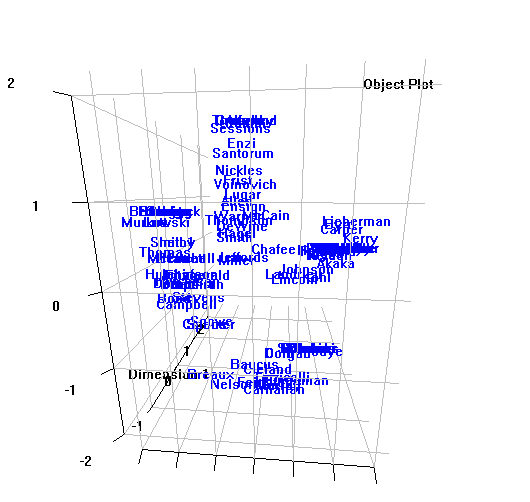
\includegraphics[height=70mm, width=70mm]{senate.png}
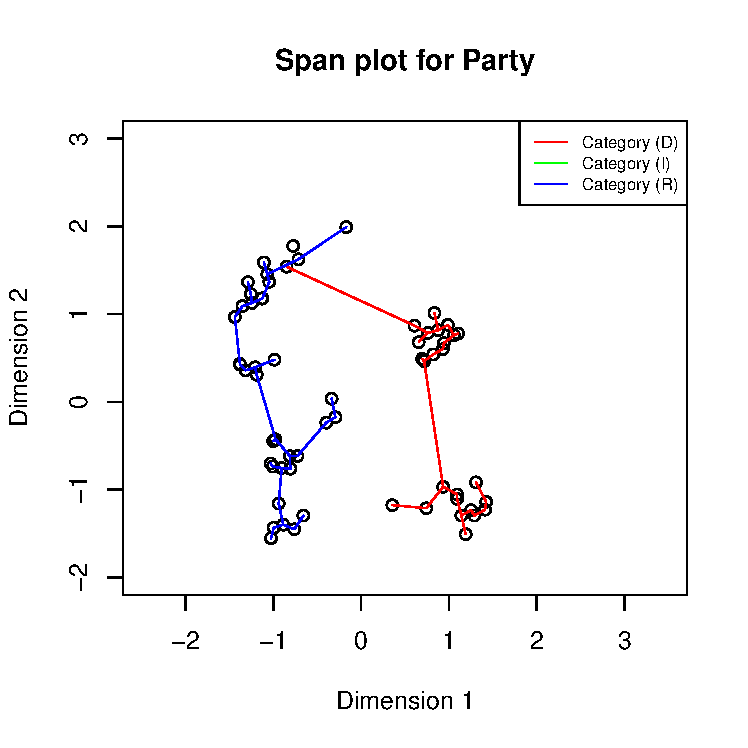
\includegraphics[height=70mm, width=70mm]{senatespan12.pdf}
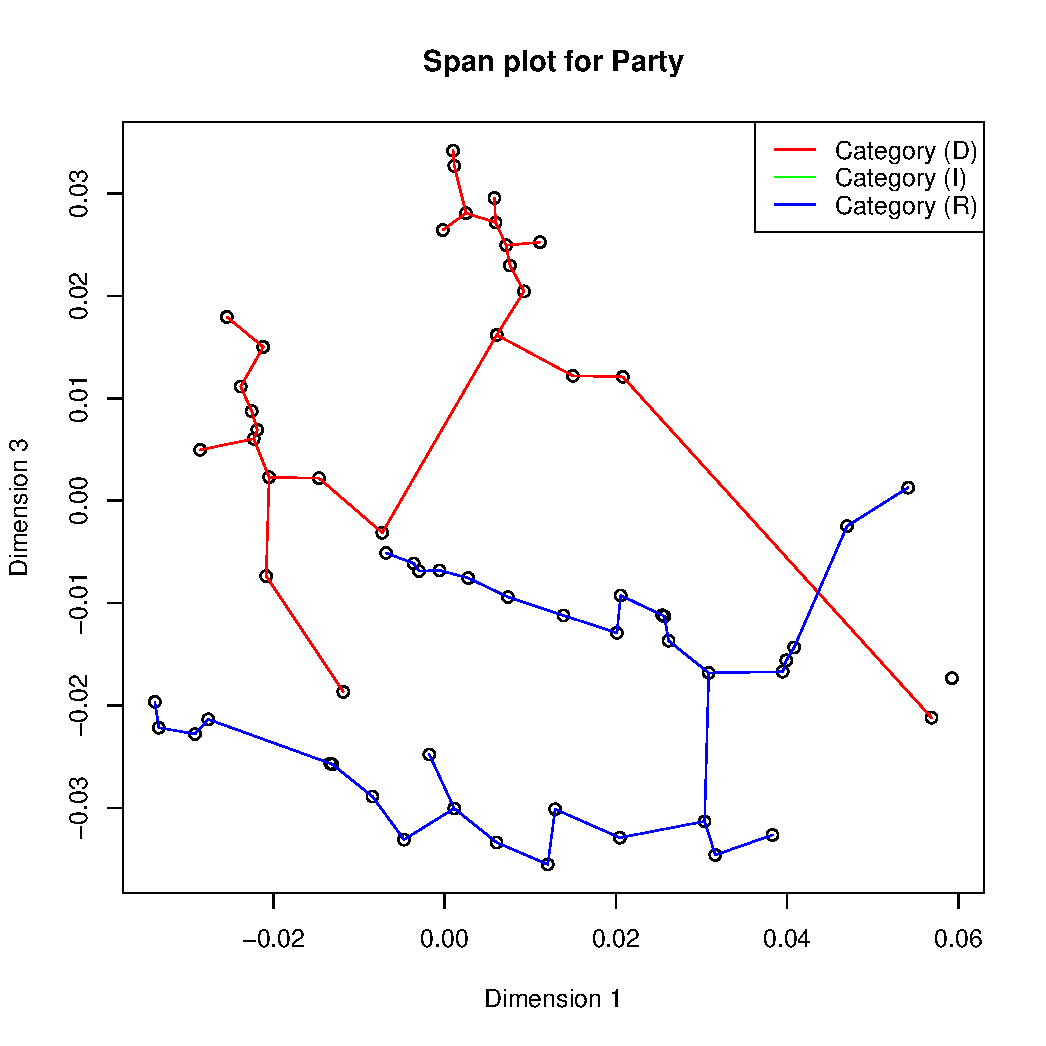
\includegraphics[height=70mm, width=70mm]{senatespan13.pdf}
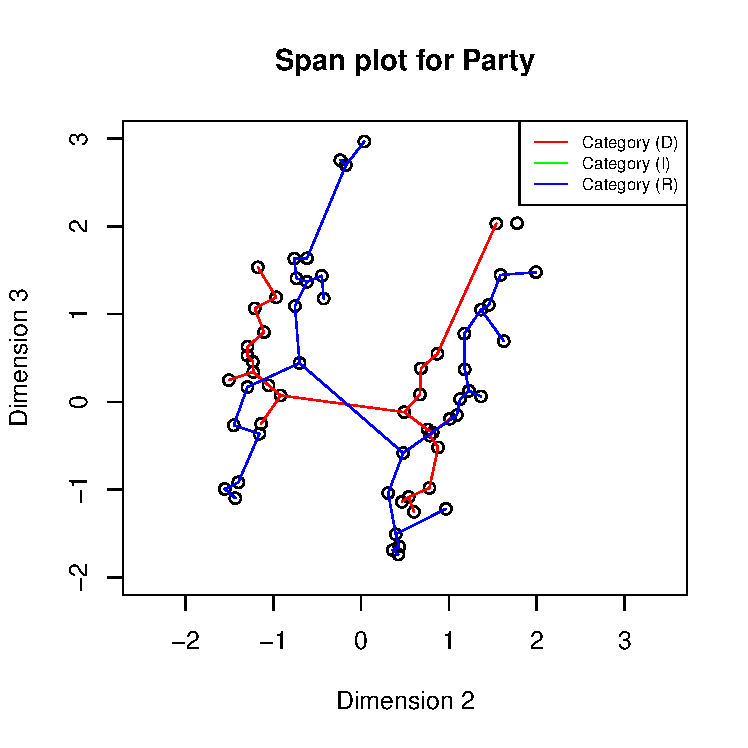
\includegraphics[height=70mm, width=70mm]{senatespan23.pdf}
\caption{\label{fig:sen} 3D Object Plot and Span Plots for Senate Dataset}
\end{center}
\end{figure}

Figure \ref{fig:sen} shows four branches (or clusters) of senators which we will denote by north, south, west and east. The west and the north branches are composed by Republicans, the east and south branches by Democrats. Note that the 3D-plot is rotated in a way that Dimension 3 is horizontally aligned, Dimension 2 is vertically aligned, and Dimension 1 is the one aligned from front to back. The two-dimensional slices show that Dimension 1 vs. 2 does not distinguish between Democrats and Republicans. If Dimension 3 is involved, as in the two bottom plots in Figure \ref{fig:sen}, the separation between Democrats and Republicans is obvious. To distinguish within north-west and south-east, respectively, Item 19 has to be taken into account:

\emph{V19: S 1438. Military Base Closures. Warner (R-VA) motion to authorize an additional round of U.S. military base realignment and closures in 2003. A ``yes'' vote is a +.} 

Republicans belonging to the north branch as well as Democrats belonging to the east branch gave a ``yes'' vote. South-Wing Democrats and West-Wing Republicans voted with ``no''. It is well known that the response on this item mainly depends on whether there is a military base in the senator's district or not; those senators who have a military base in their district do not want to close it since such a base provides working places and is an important income source for the district. Hence, this is the determining factor and not the party affiliation of the senator. This result is underpinned by Figure \ref{fig:senload} where Item 19 is clearly separated from the remaining items.

\begin{figure}[ht]
\begin{center}
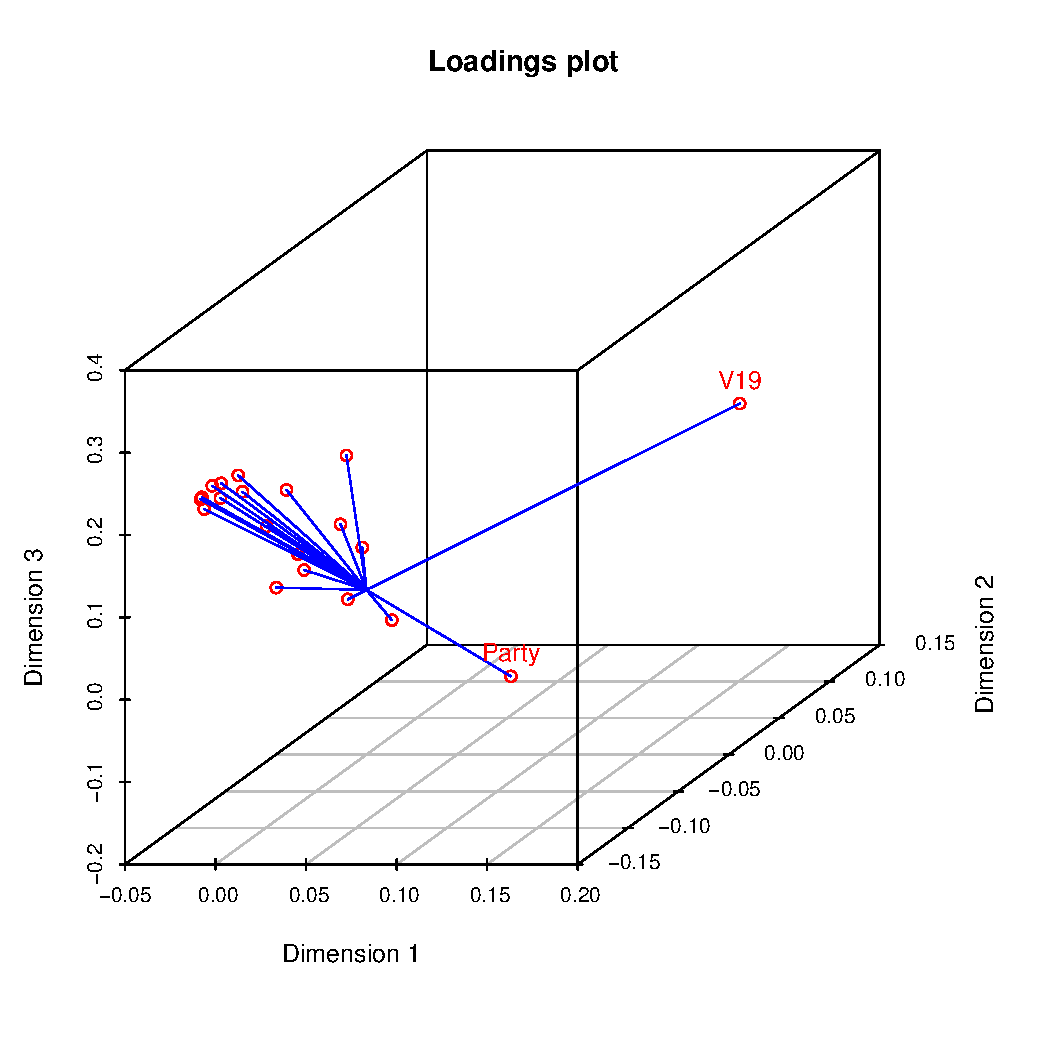
\includegraphics[height=85mm, width=85mm]{senateload.pdf}
\caption{\label{fig:senload} Loadings Plot for Senate Dataset}
\end{center}
\end{figure}

Given a (multiple) homals solution, we can reconstruct the indicator matrix by assigning each object to the closest points of the variable.

\begin{Schunk}
\begin{Sinput}
> p.res <- predict(res)
> p.res$cl.table$Party
\end{Sinput}
\begin{Soutput}
     pre
obs   (D) (I) (R)
  (D)  49   1   0
  (I)   0   1   0
  (R)   0   8  41
\end{Soutput}
\end{Schunk}

From the classification table we see that 91\% of the party affiliations are correctly classified. Note that in the case of such a simple homals solution it can happen that a lower dimensional solution results in a better classification rate than a higher dimensional. The reason is that in simple homals the classification rate is not the criterion to be optimized. 

\newpage
\subsection{Predictive Models and Canonical Correlation}
\label{sec:pmcca}
The \code{sets} argument allows for partitioning the variables into sets in order to emulate canonical correlation analysis and predictive models. As outlined above, if the variables are partitioned into asymmetric sets of one variable vs. the others, we can put this type of homals model into a predictive modeling context. If not, the interpretation in terms of canonical correlation is more appropriate. 

\begin{figure}[hbt]
\begin{center}
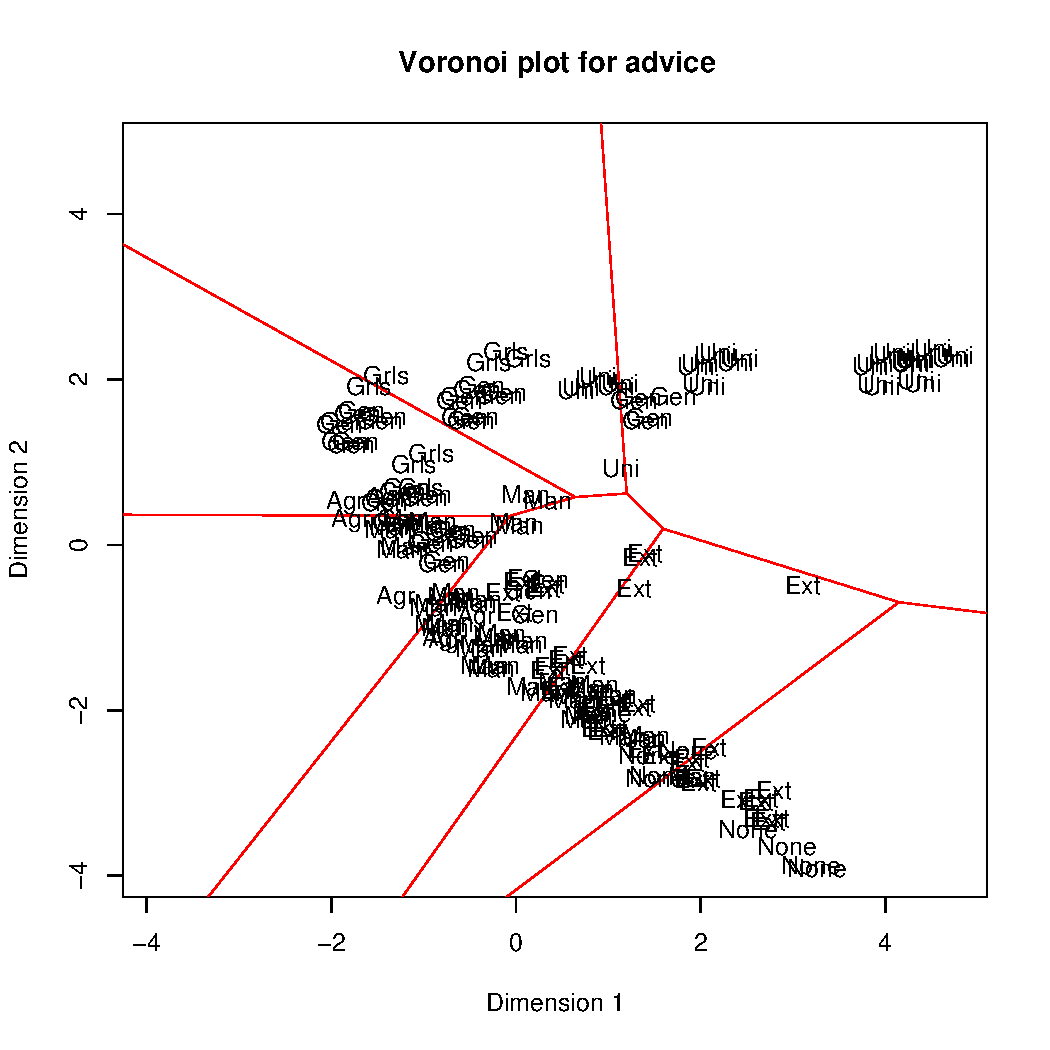
\includegraphics[height=75mm, width=75mm]{galoVor.pdf}
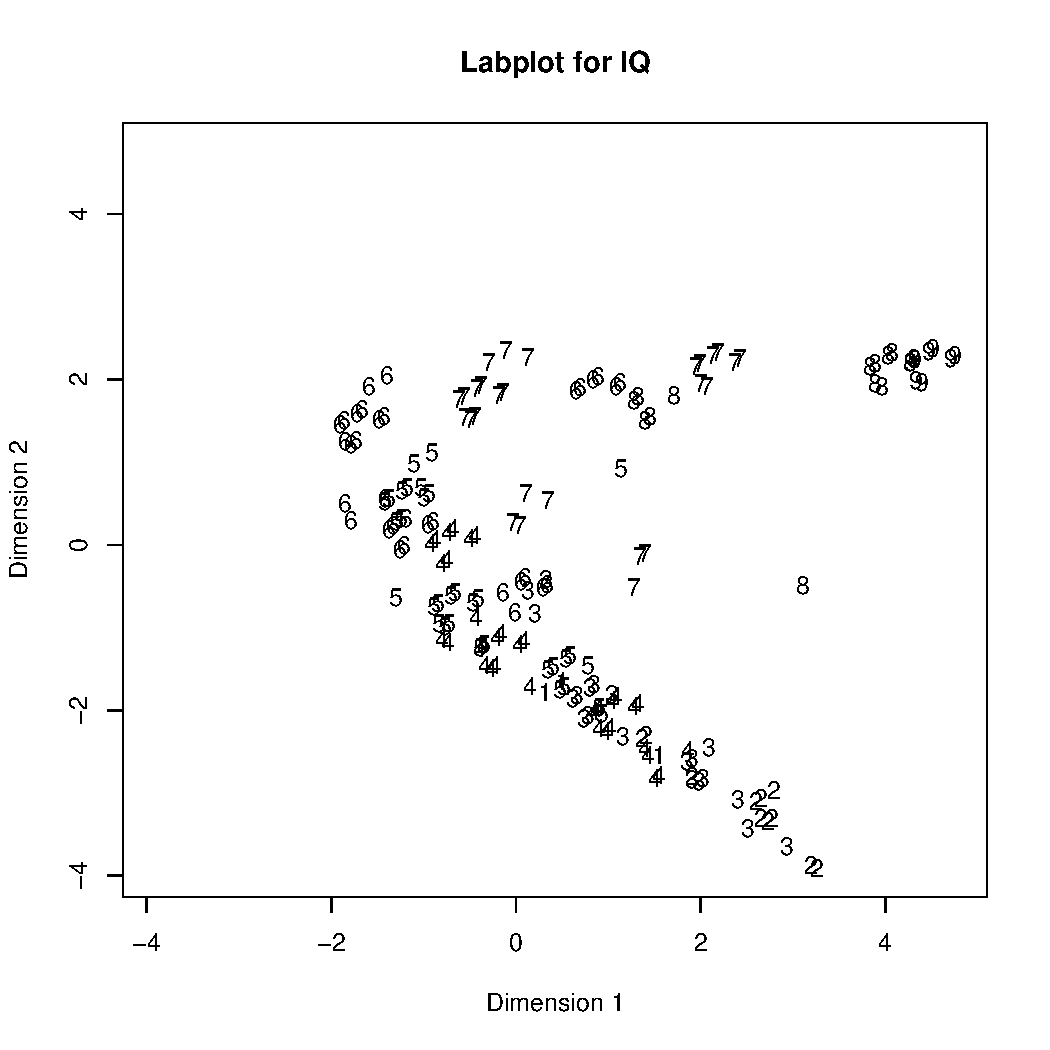
\includegraphics[height=75mm, width=75mm]{galoLab.pdf}
\caption{\label{fig:vor}Voronoi Plot and Label Plot for Galo Data}
\end{center}
\end{figure}

To demonstrate this, we use the \code{galo} dataset \citep{Peschar:75} where data of 1290 school children in the sixth grade of an elementary school in the city of Groningen (Netherlands) were collected. The variables are Gender, IQ (categorized into 9 ordered categories), Advice (teacher categorized the children into 7 possible forms of secondary education, i.e., Agr = agricultural; Ext = extended primary education; Gen = general; 
Grls = secondary school for girls; Man = manual, including housekeeping; 
None = no further education; Uni = pre-University) and SES (parent's profession in 6 categories). In this example it could be of interest to predict Advice from Gender, IQ, and SES.

\begin{Schunk}
\begin{Sinput}
> data(galo)
> res <- homals(galo, active = c(rep(TRUE, 4), FALSE),
+ sets = list(c(1, 2, 4), 3, 5))
> plot(res, plot.type = "vorplot", var.subset = 3)
> plot(res, plot.type = "labplot", var.subset = 2)
> predict(res)
\end{Sinput}
\begin{Soutput}
Classification rate:
  Variable Cl. Rate %Cl. Rate
1   gender   0.5690     56.90
2       IQ   0.6341     63.41
3   advice   0.6310     63.10
4      SES   0.2907     29.07
5   School   0.0132      1.32
\end{Soutput}
\end{Schunk}

A rate of .6318 correctly classified teacher advice results. The Voronoi plot in Figure \ref{fig:vor} shows the Voronoi regions for the same variable. A labeled plot is given for the IQs which shows that on the upper half of the horseshoe there are mainly children with IQ-categories 7-9. Distinctions between these levels of intelligence are mainly reflected by Dimension 1. For the lower horseshoe half it can be stated that both dimensions reflect differences in lower IQ-categories.

Using the classical iris dataset, the aim is to predict Species from Petal/Sepal Length/Width. The polynomial level constraint is posed on the predictors and the response is treated as nominal. A hull plot for the response, a label plot Petal Length and loss plots for all predictors are produced.

\begin{Schunk}
\begin{Sinput}
> data(iris)
> res <- homals(iris, sets = list(1:4, 5),
+ level = c(rep("polynomial", 4), "nominal"), rank = 2,
+ itermax = 2000)
> plot(res, plot.type = "hullplot", var.subset = 5, cex = 0.7,
+ xlim = c(-3, 3), ylim = c(-3, 3))
> plot(res, plot.type = "labplot", var.subset = 3, cex = 0.7,
+	xlim = c(-3, 3), ylim = c(-3, 3))
> plot(res, plot.type = "lossplot", var.subset = 1:4, cex = 0.7,
+	xlim = c(-3, 4), ylim = c(-3, 4))
\end{Sinput}
\end{Schunk}

\begin{figure}[hbt]
\begin{center}
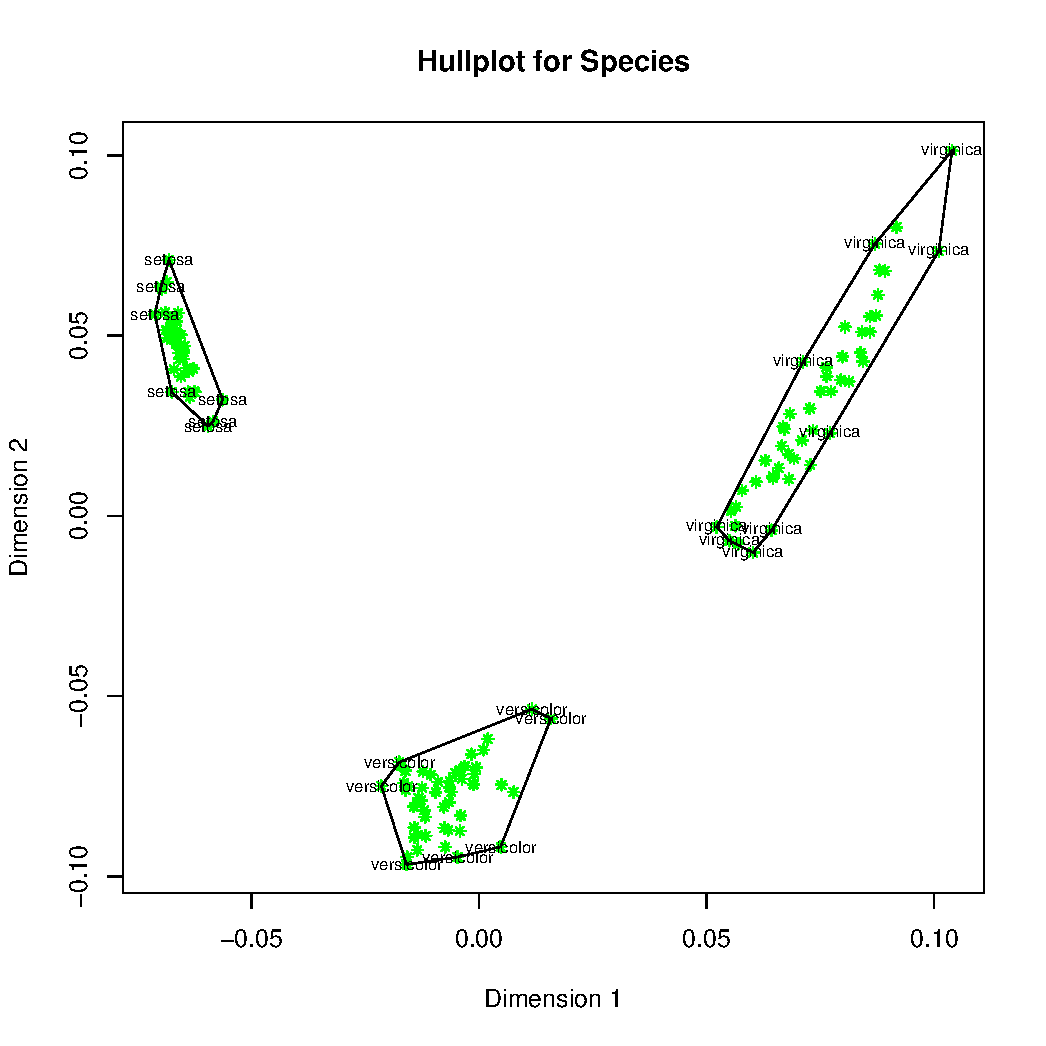
\includegraphics[height=75mm, width=75mm]{irisHull.pdf}
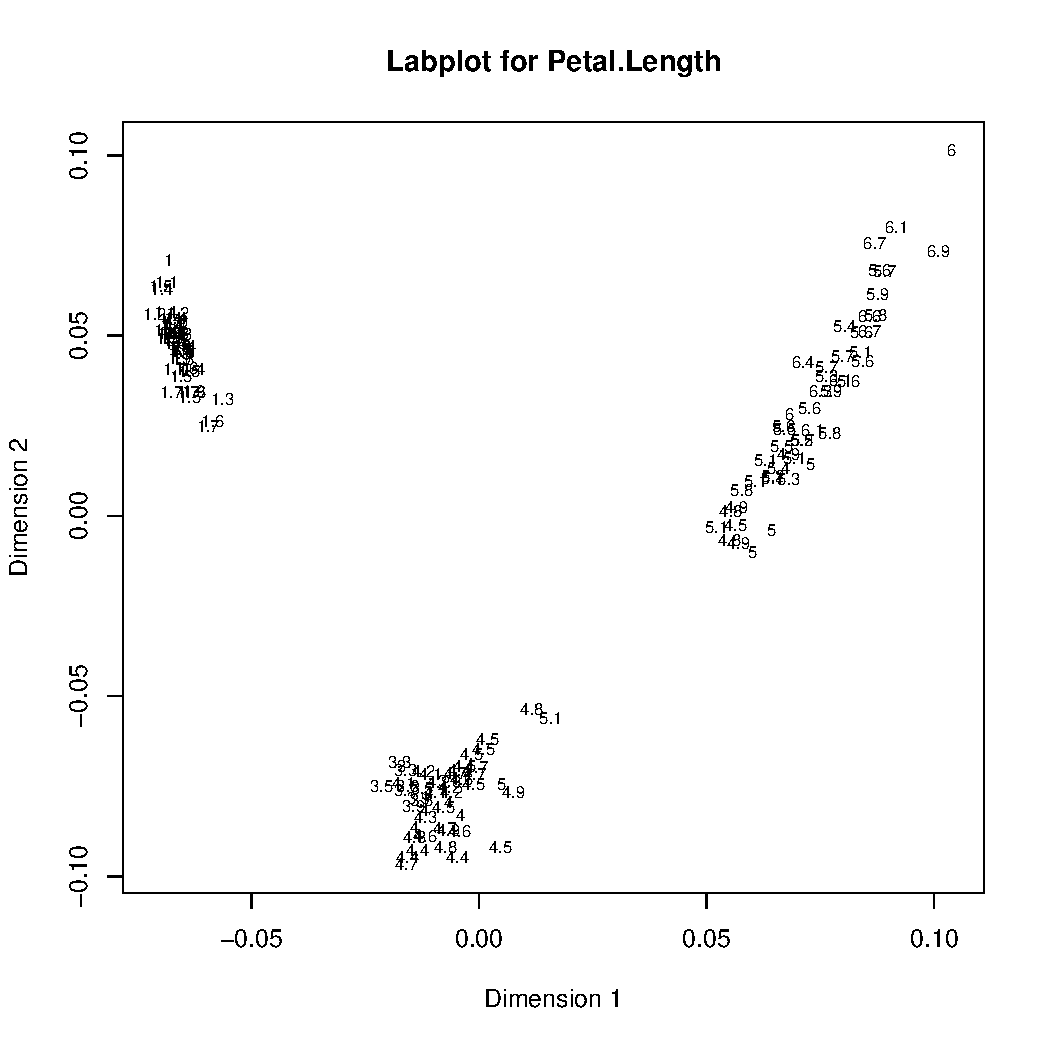
\includegraphics[height=75mm, width=75mm]{irisLab.pdf}
\caption{\label{fig:iris}Hullplot and Label Plot for Iris Data}
\end{center}
\end{figure}

For this two-dimensional homals solution, 100\% of the iris species are correctly classified. The hullplot in Figure \ref{fig:iris} shows that the species are clearly separated on the two-dimensional plane. In the label plot the object scores are labeled with the response on Petal Length and it becomes obvious that small lengths form the setosa ``cluster", whereas iris virginica are composed by obervations with large petal lengths. Iris versicolor have medium lengths. 

The loss plots in Figure \ref{fig:irisLoss} show the fitted rank-2 solution (red lines) against the unrestricted solution. The implication of the polynomial level restriction for the fitted model is obvious.

\begin{figure}[hbt]
\begin{center}
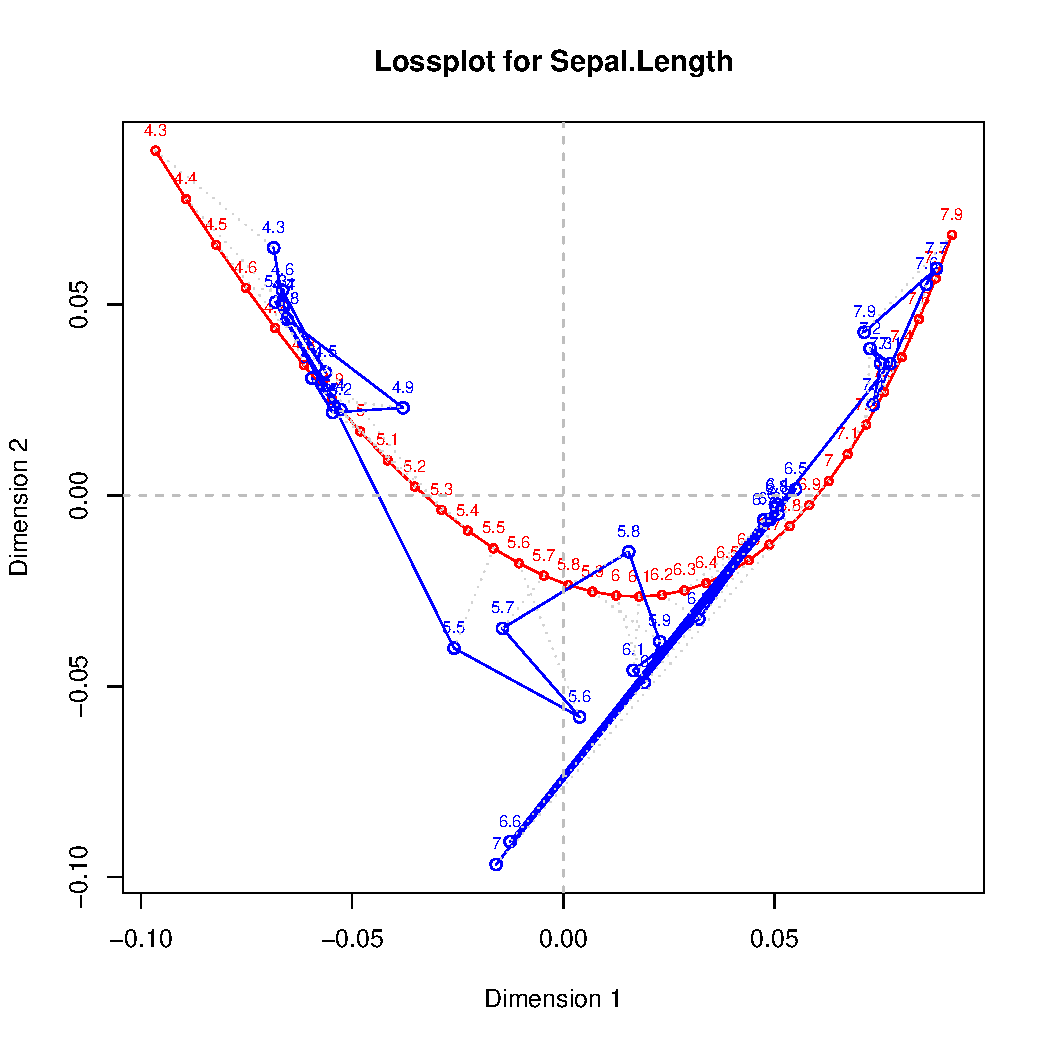
\includegraphics[height=70mm, width=70mm]{irisLoss1.pdf}
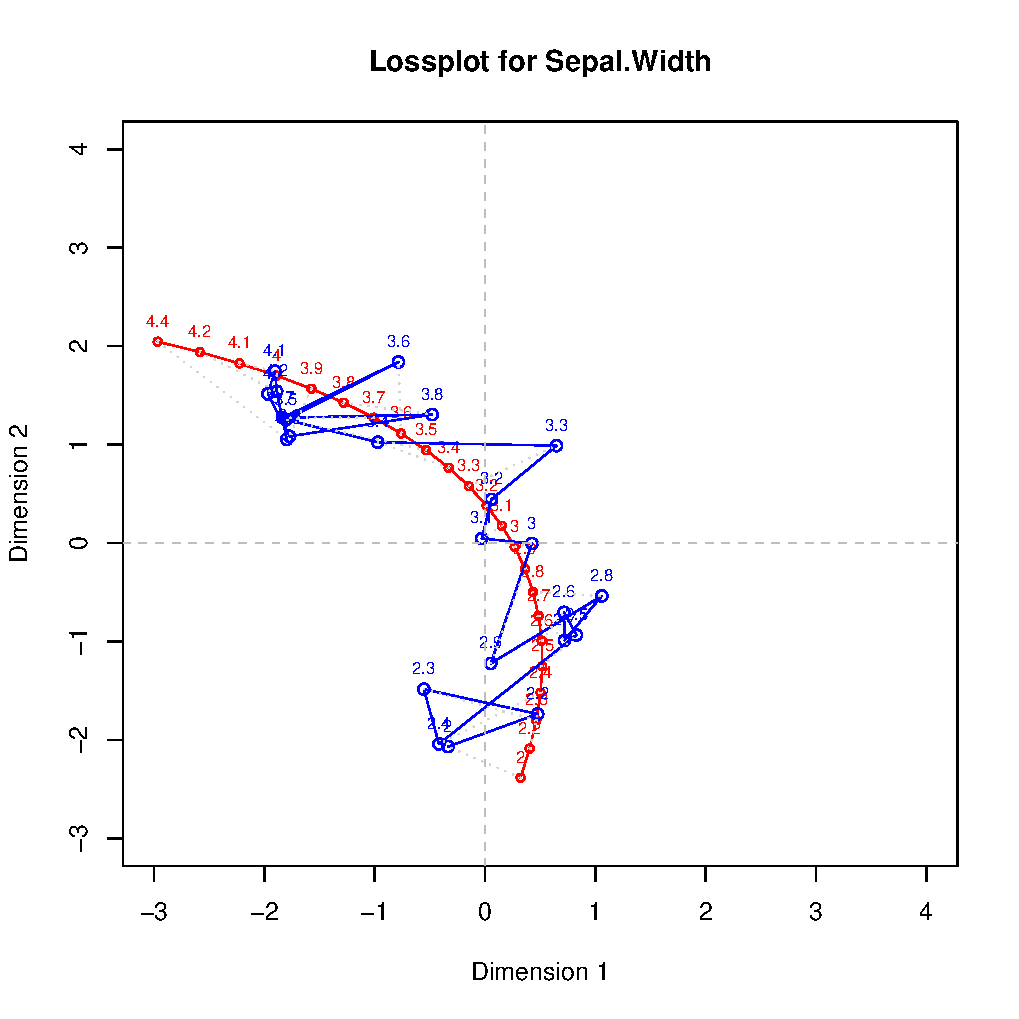
\includegraphics[height=70mm, width=70mm]{irisLoss2.pdf}
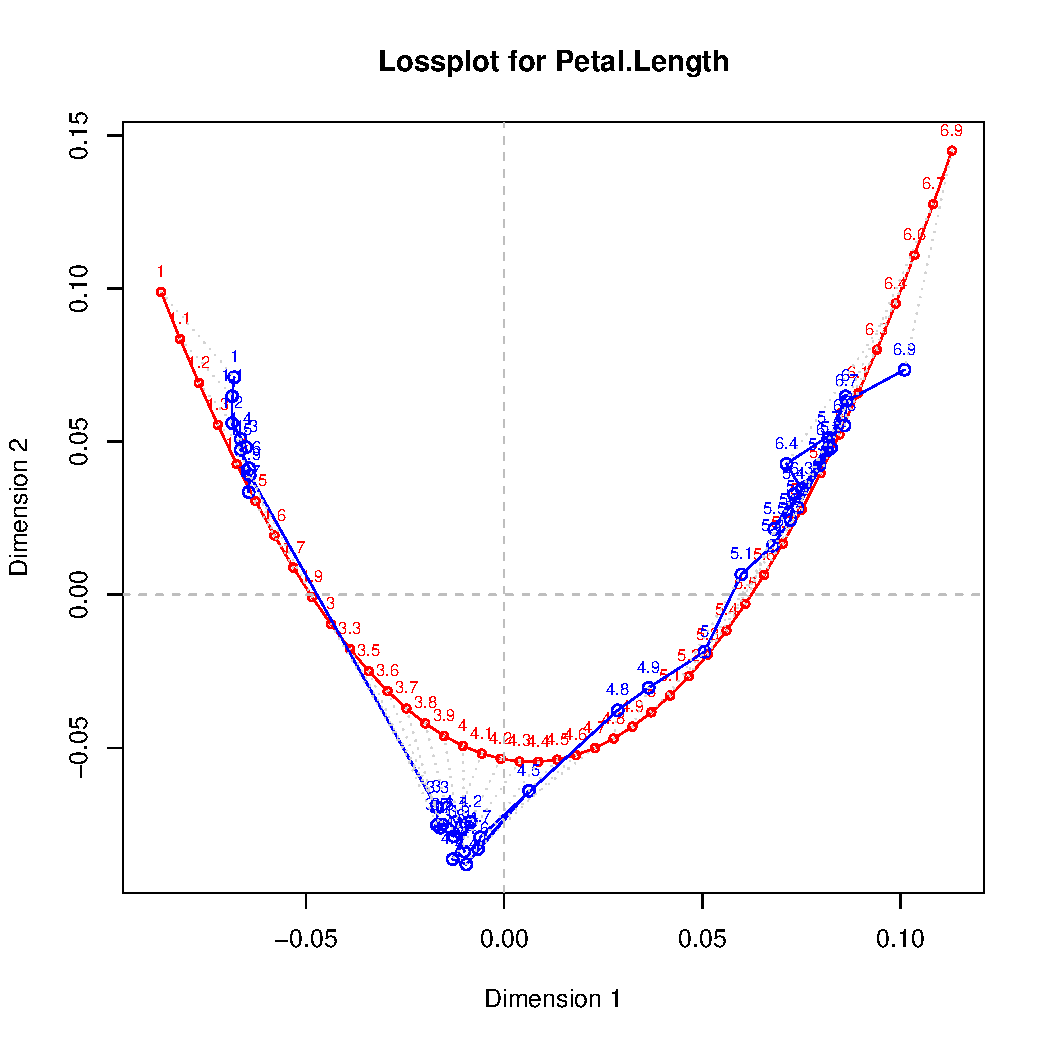
\includegraphics[height=70mm, width=70mm]{irisLoss3.pdf}
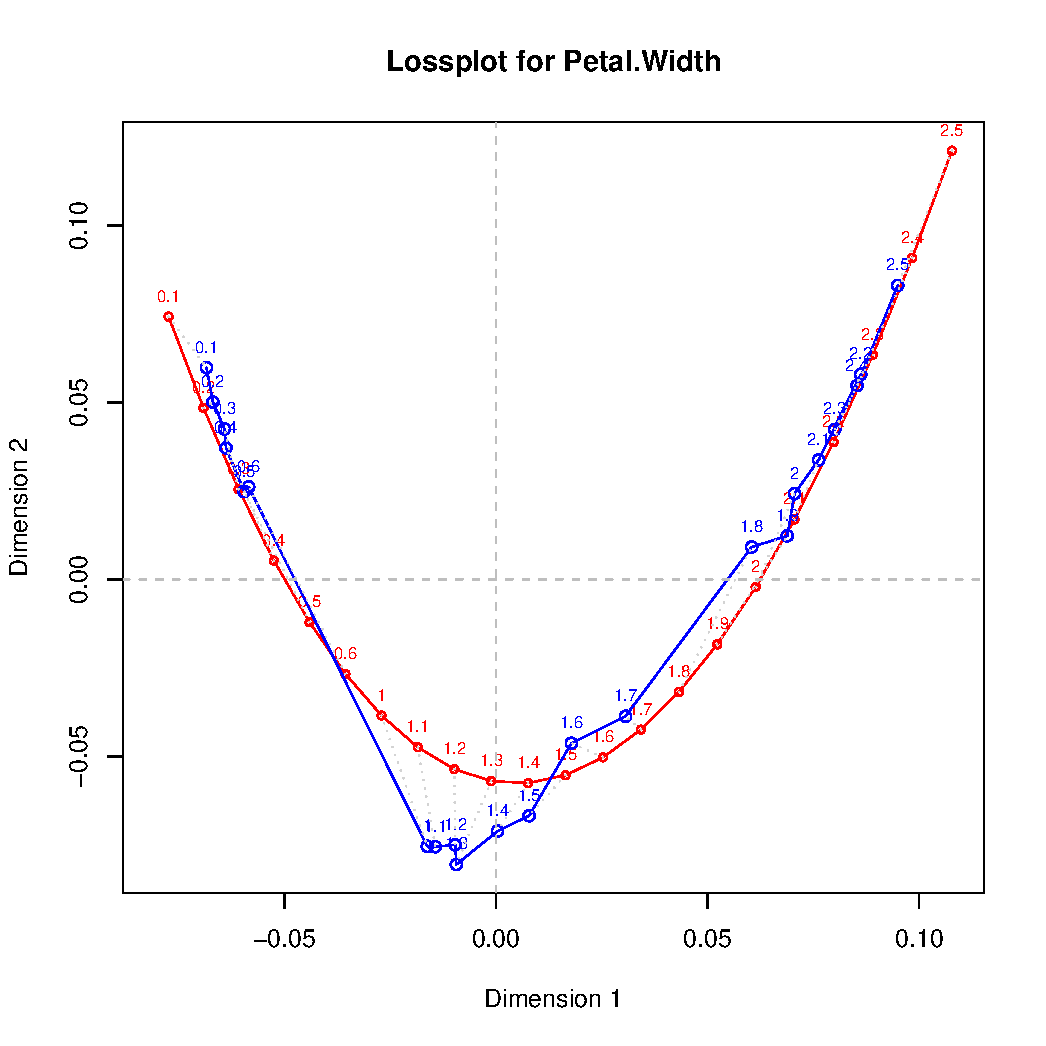
\includegraphics[height=70mm, width=70mm]{irisLoss4.pdf}
\caption{\label{fig:irisLoss}Loss plots for Iris Predictors}
\end{center}
\end{figure}

To show another homals application of predictive (in this case regression) modeling we use the Neumann dataset \citep{Wilson:26}: Willard Gibbs discovered a theoretical formula connecting the density, the
pressure, and the absolute temperature of a mixture of gases with convertible 
components. He applied this formula and the estimated constants to 65 experiments
carried out by Neumann, and he discusses the systematic and accidental divergences (residuals). In \pkg{homals} such a linear regression problem can be emulated by setting numerical levels. Constraining the levels to be ordinal, we get a monotone regression \citep{Gifi:90}. 

\begin{Schunk}
\begin{Sinput}
> data(neumann)
> res.lin <- homals(neumann, sets = list(3, 1:2), level = "numerical", rank = 1)
> res.mon <- homals(neumann, sets = list(3, 1:2), level = "ordinal", rank = 1)
> plot(res.lin, plot.type = "loadplot", main = "Loadings Plot Linear Regression",
+ xlim = c(-10, 10), ylim = c(-10, 10))
> plot(res.mon, plot.type = "loadplot", main = "Loadings Plot Monotone Regression",
+ xlim = c(-10, 10), ylim = c(-10, 10))
\end{Sinput}
\end{Schunk}

The points in the loadings plot in Figure \ref{fig:neuload} correspond to regression coefficients.

\begin{figure}[hbt]
\begin{center}
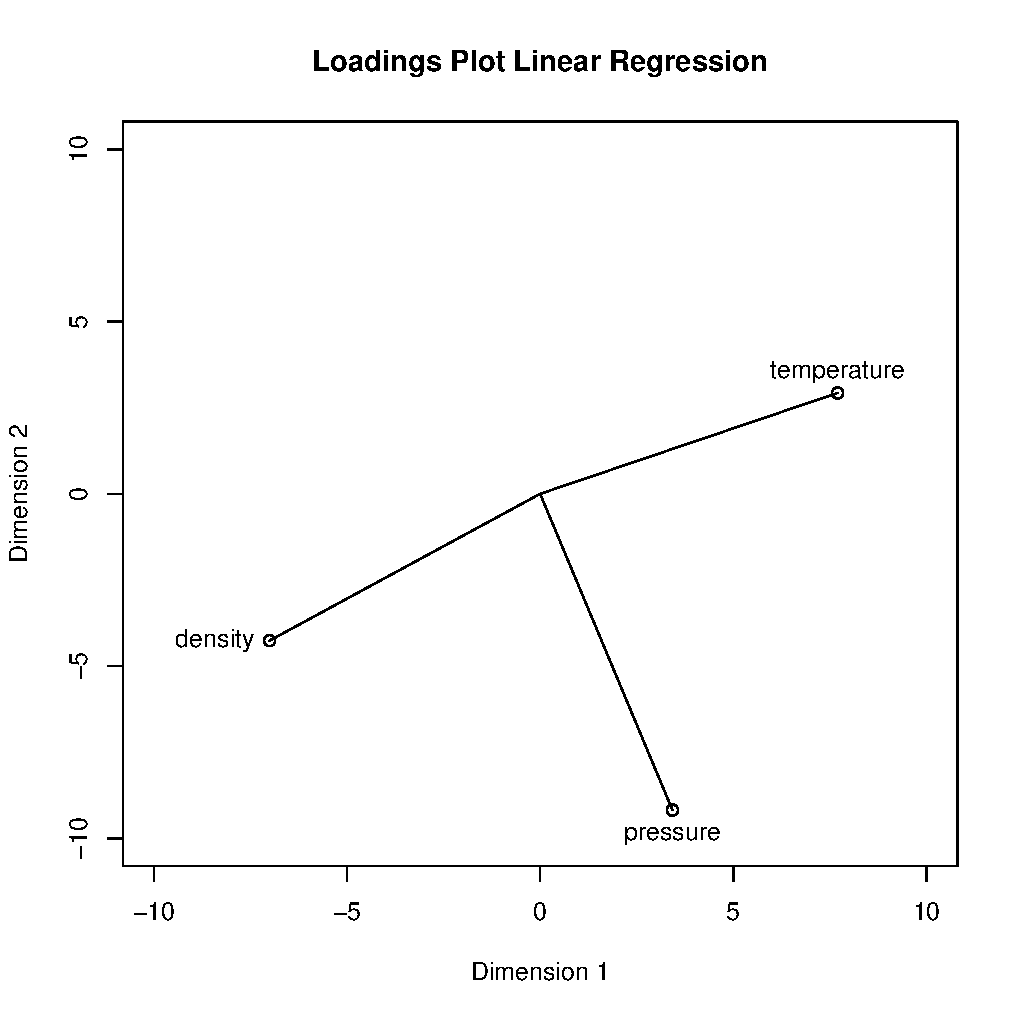
\includegraphics[height=70mm, width=70mm]{neuloadlin.pdf}
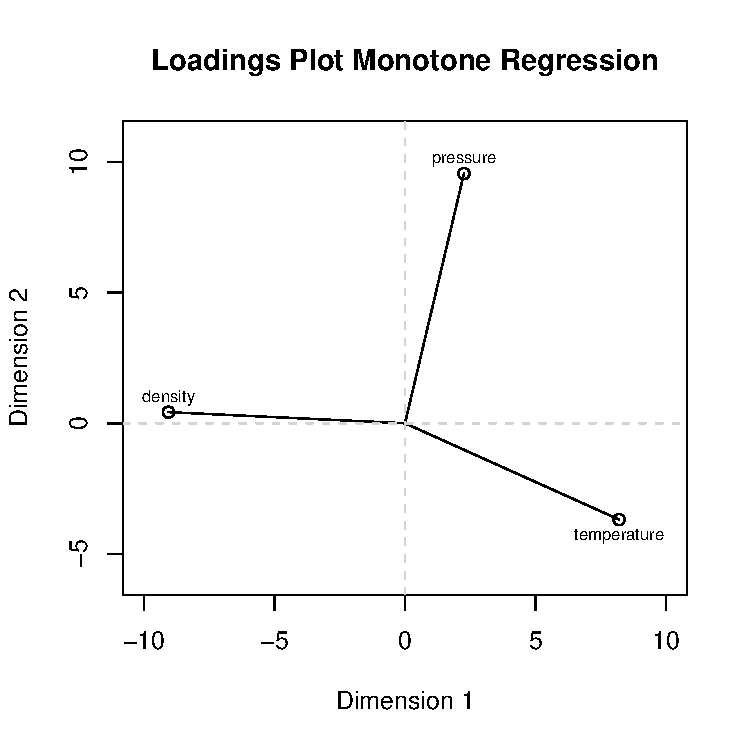
\includegraphics[height=70mm, width=70mm]{neuloadmon.pdf}
\caption{\label{fig:neuload}Loading Plots for Neumann Regression}
\end{center}
\end{figure}

The impact of the level restrictions on the scaling is visualized in the transformation plots in Figure \ref{fig:neutrf}. Numerical level restrictions lead to linear transformations of the original scale with respect to the homals scaling (i.e. linear regression). Pertaining to ordinal levels, monotone transformations are carried out (i.e. monotone regression). 

\begin{figure}[hbt]
\begin{center}
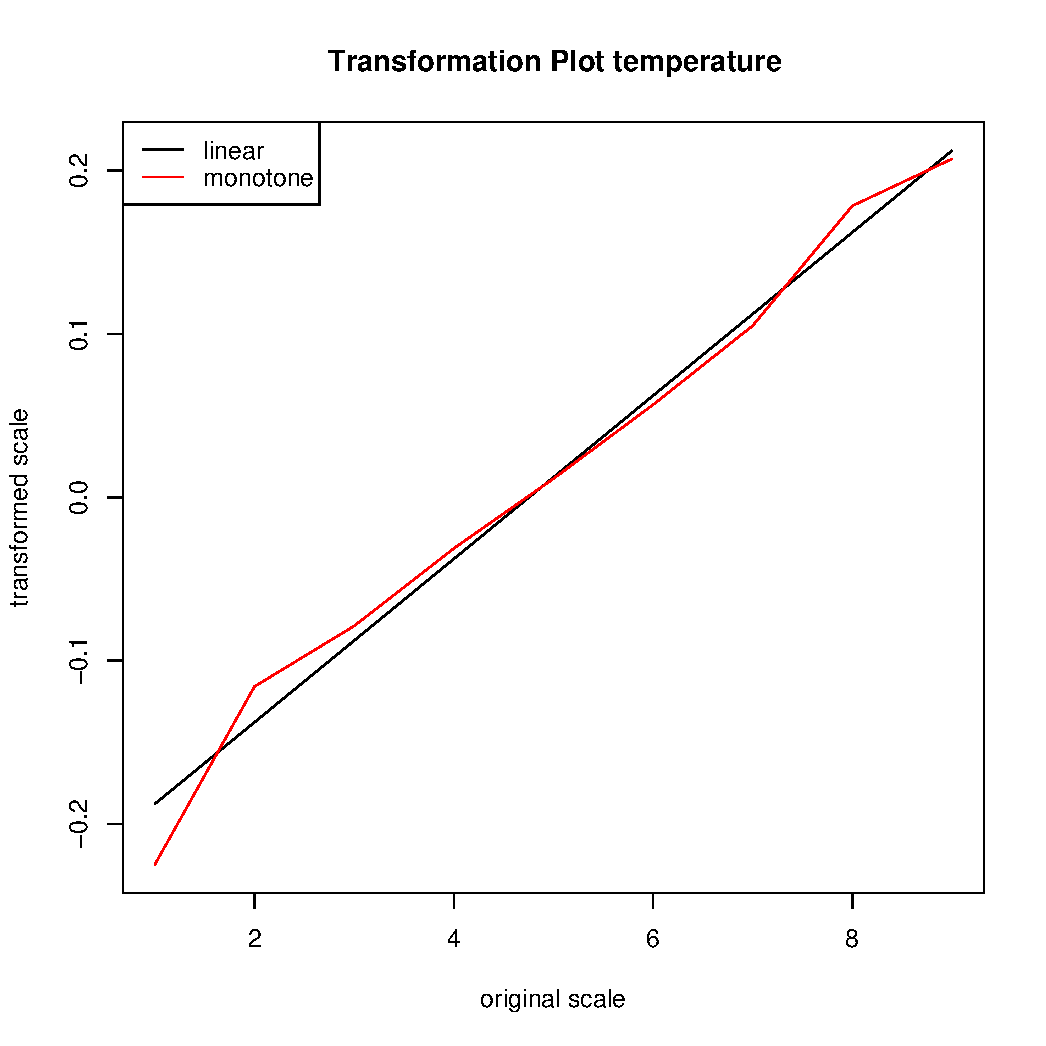
\includegraphics[height=60mm, width=60mm]{neutrftemp.pdf}
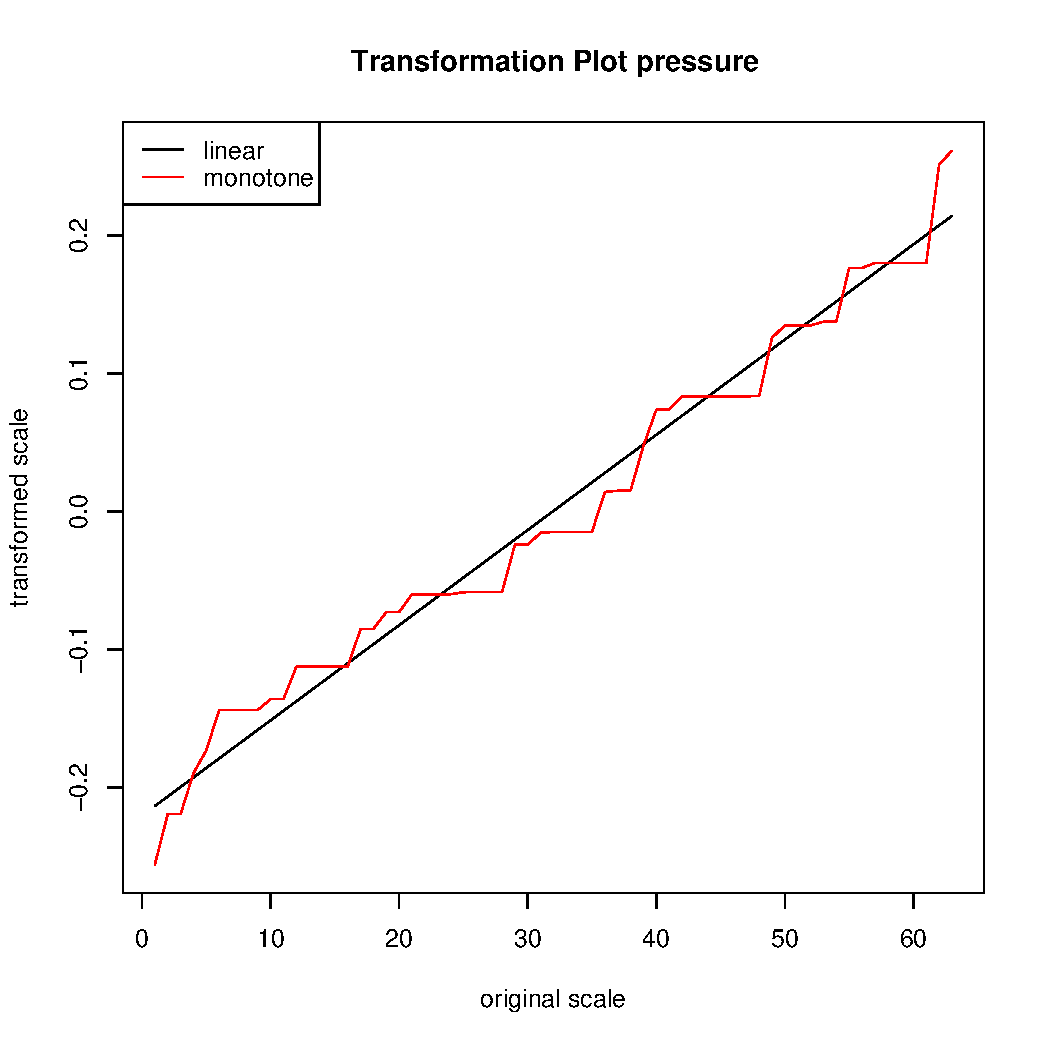
\includegraphics[height=60mm, width=60mm]{neutrfpres.pdf}
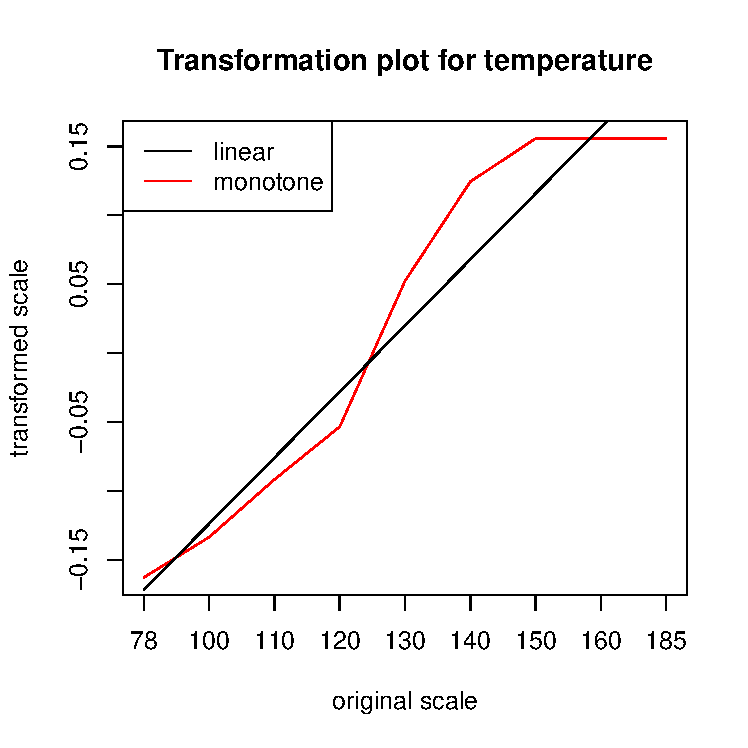
\includegraphics[height=60mm, width=60mm]{neutrfdens.pdf}
\caption{\label{fig:neutrf}Transformation Plots for Neumann Regression}
\end{center}
\end{figure}

\subsection{NLPCA on Roskam data}
\label{sec:pcex}
\citet{Roskam:68} collected preference data where 39 psychologists ranked all nine areas (see Table \ref{tab:area}) of the Psychology Department at the University of Nijmengen. 

\begin{table}[ht]
\centering
\begin{tabular}{|c|l|}
\hline
SOC& Social Psychology\\
EDU& Educational and Developmental Psychology\\
CLI& Clinical Psychology\\
MAT& Mathematical Psychology and Psychological Statistics\\
EXP& Experimental Psychology\\
CUL& Cultural Psychology and Psychology of Religion\\
IND& Industrial Psychology\\
TST& Test Construction and Validation\\
PHY& Physiological and Animal Psychology\\
\hline
\end{tabular}
\caption{\label{tab:area}Psychology Areas in Roskam Data.}
\end{table}

Using this data set we will perform two-dimensional NLPCA by restricting the rank to be 1. Note that the objects are the areas and the variables are the psychologists. Thus, the input data structure is a $9 \times 39$ data frame. Note that the scale level is set to ``ordinal".

\begin{Schunk}
\begin{Sinput}
> data(roskam)
> res <- homals(roskam, rank = 1, level = "ordinal")
> plot(res, plot.type = "objplot", xlim = c(-2.5, 2.5), ylim = c(-2.5, 2.5))
> plot(res, plot.type = "vecplot", var.subset = 2, main = "Vector Plot Rater 2",
+ xlim = c(-2.5, 2.5), ylim = c(-2.5, 2.5))
\end{Sinput}
\end{Schunk}

\begin{figure}[hbt]
\begin{center}
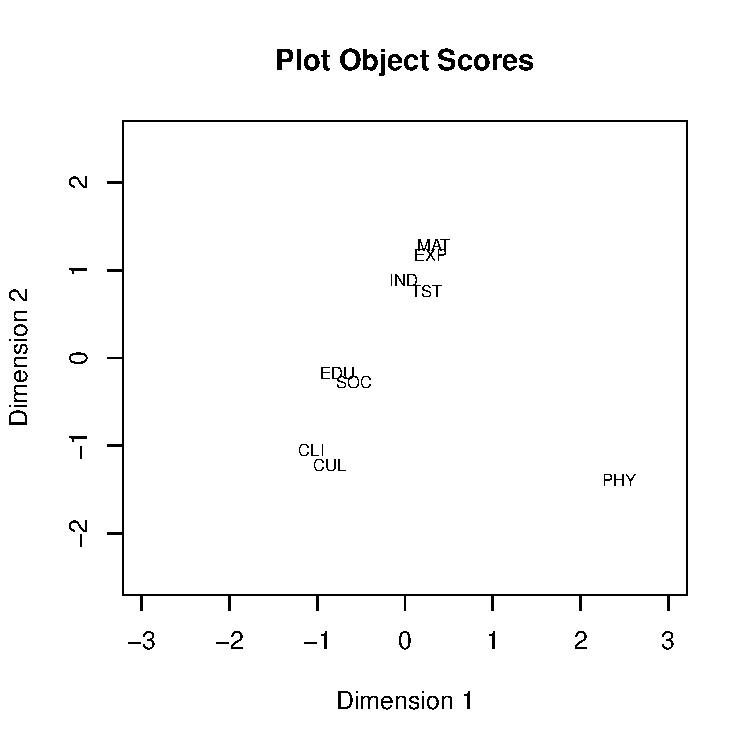
\includegraphics[height=75mm, width=75mm]{roskamobj.pdf}
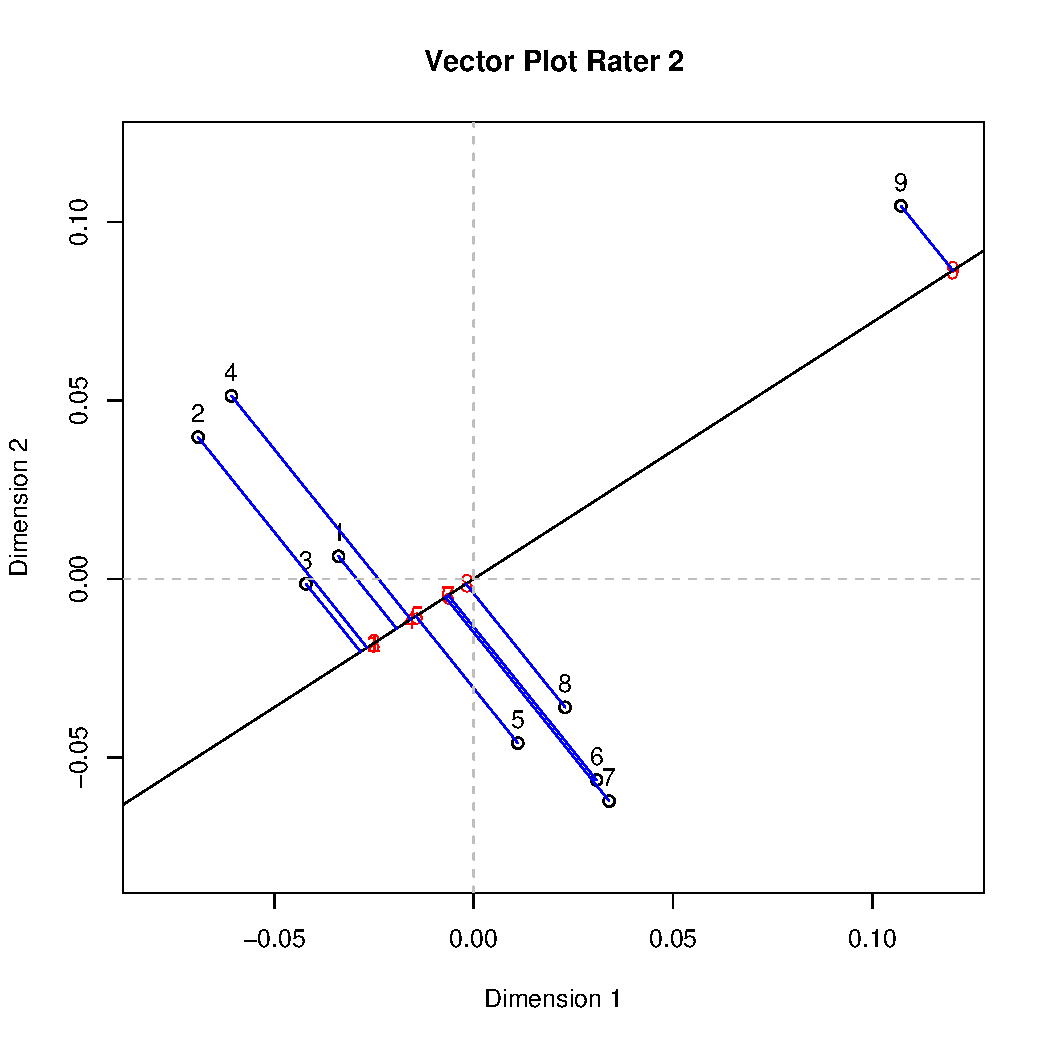
\includegraphics[height=75mm, width=75mm]{roskamvec.pdf}
\caption{\label{fig:roskam}Plots for Roskam data}
\end{center}
\end{figure}

The object plot in Figure \ref{fig:roskam} shows interesting rating ``twins" of departmental areas: mathematical and experimental psychology, industrial psychology and test construction (both are close to the former two areas), educational and social psychology, clinical and cultural psychology. Physiological and animal psychology are somewhat separated from the other areas. Obviously this rater is attracted to areas like social, cultural and clinical psychology rather than to methodological fields. 
The vector plot on the right hand side projects the category scores onto a straight line determined by rank restricted category quantifications. Similarly, a projection plot could be created. Further analyses of this dataset within a PCA context can be found in \citet{deLeeuw:06}. 
 
\section{Discussion}
In this paper theoretical foundations of the methodology used in \pkg{homals} are elaborated and package application and visualization issues are presented. Basically, \pkg{homals} covers the techniques described in \citet{Gifi:90}: Homogeneity analysis, NLCCA, predictive models, and NLPCA. It can handle missing data and the scale level of the variables can be taken into account. The package offers a broad variety of real-life datasets and furthermore provides numerous methods of visualization, either in a two-dimensional or in a three-dimensional way. Future enhancements will be to replace indicator matrices by more general B-spline bases and to incorporate weights for observations. To conclude, \pkg{homals} provides flexible, easy-to-use routines which allow researchers from different areas to compute, interpret, and visualize methods belonging to the Gifi-family. 

\bibliography{homalsR}

\end{document}

